\documentclass[../Ansoegning.tex]{subfiles}
\begin{document}
%-------------------------------------------------------------------------
\begin{center}
    \textbf{\LARGE{Boligudgift}}\vspace{-3ex}
\end{center}

Jeg er på nuværende tidspunkt midlertidigt bosat i Frankrig i forbindelse med at jeg tager min 5. semesters ingeniørpraktik ved CERN i Schweiz. Herunder fremgår transaktionsdokument for min boligudgifter. Her har jeg lejet mig ind i et værelse med en samlet månedlig udgift på 780 CHF = 885 EUR = 5819 DKK. Dette beløb dækker vand, varme og el: 
% Side 1:
\begin{minipage}{1\textwidth}
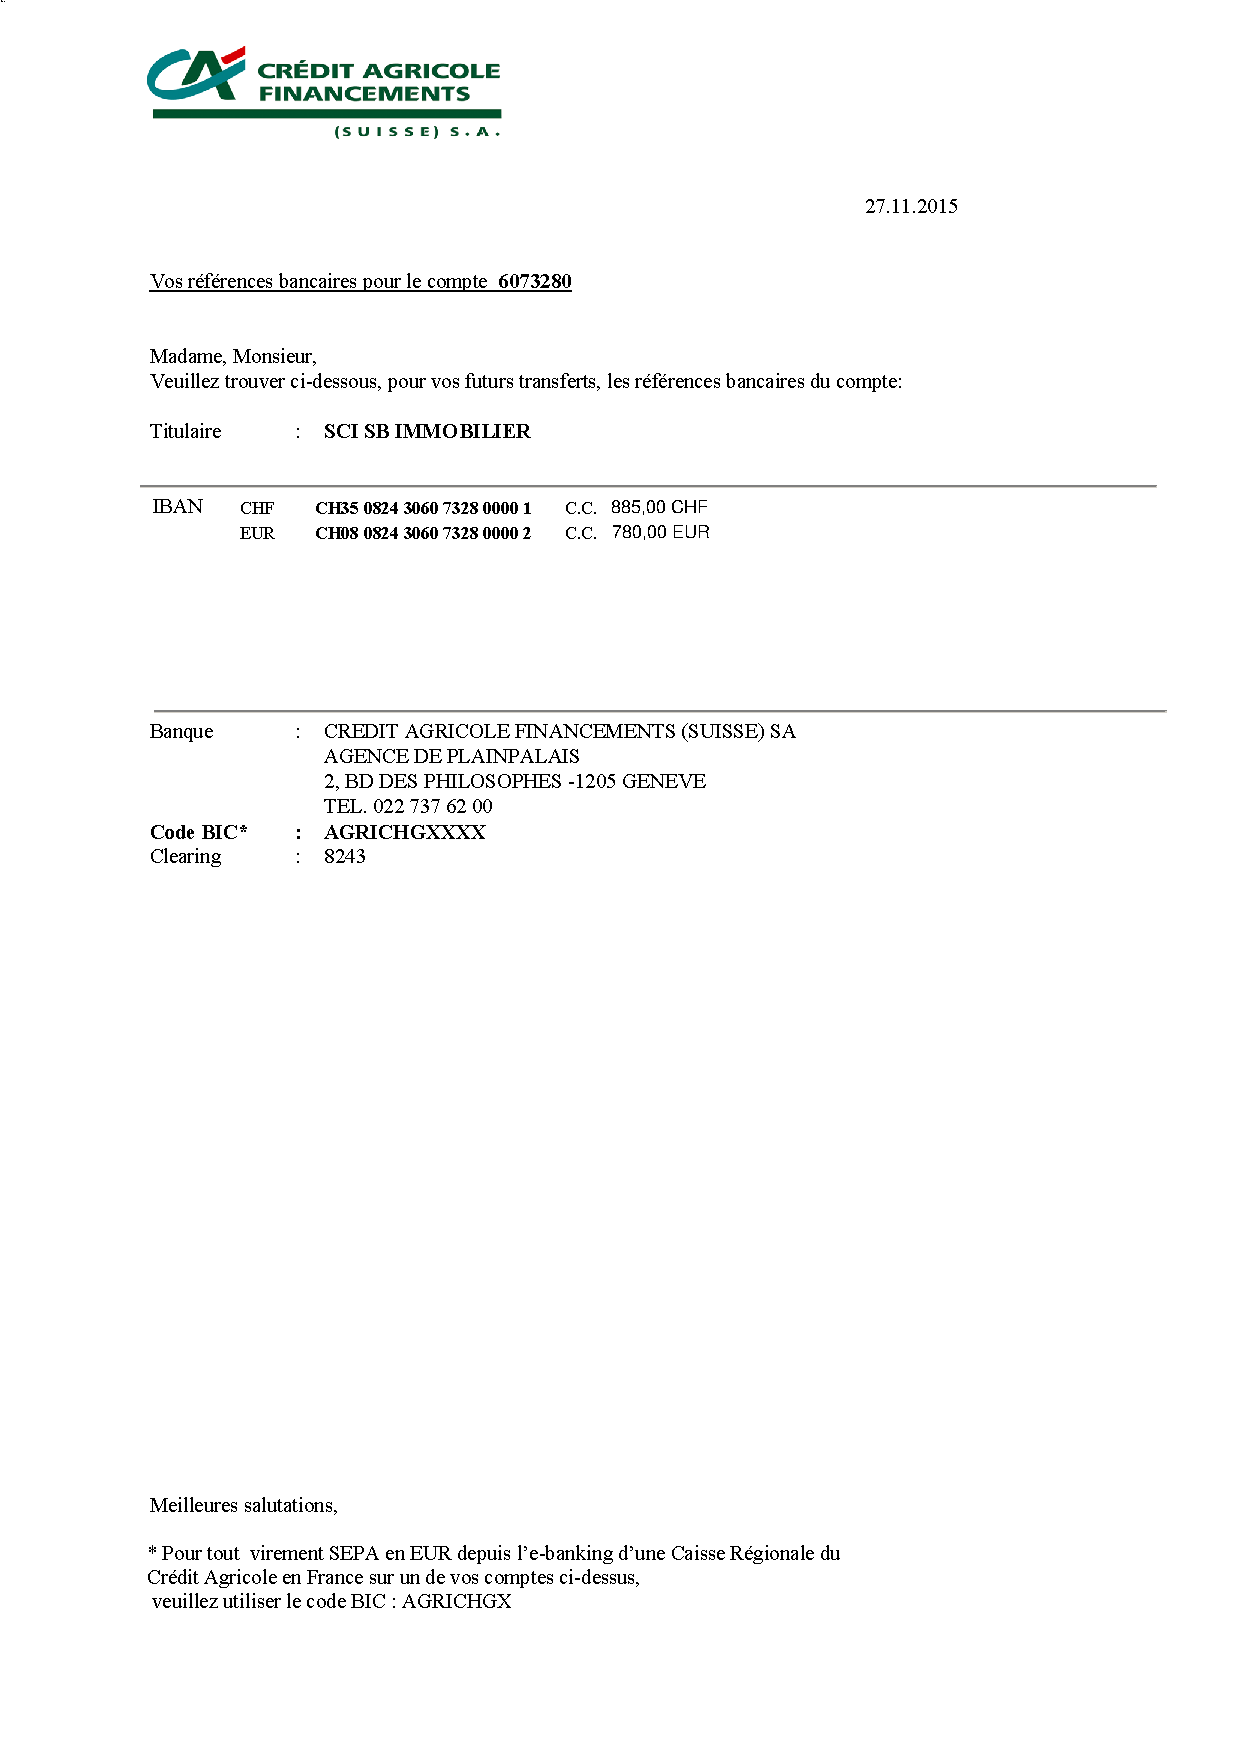
\includepdf[pages={1}, scale=.8, pagecommand={\label{sec:flaskehaeldning}}, offset=0 -2cm]{Eksterne_filer/leje.pdf}
\end{minipage}
    \newpage

Figuren herunder er en mailkorrespondance med min udlejer i Frankrig, Armand Jost. Her bekræfter han, at beløbet på 780 EUR dækker husleje samt vand, varme og el:
\begin{figure}[H]
	\centering
	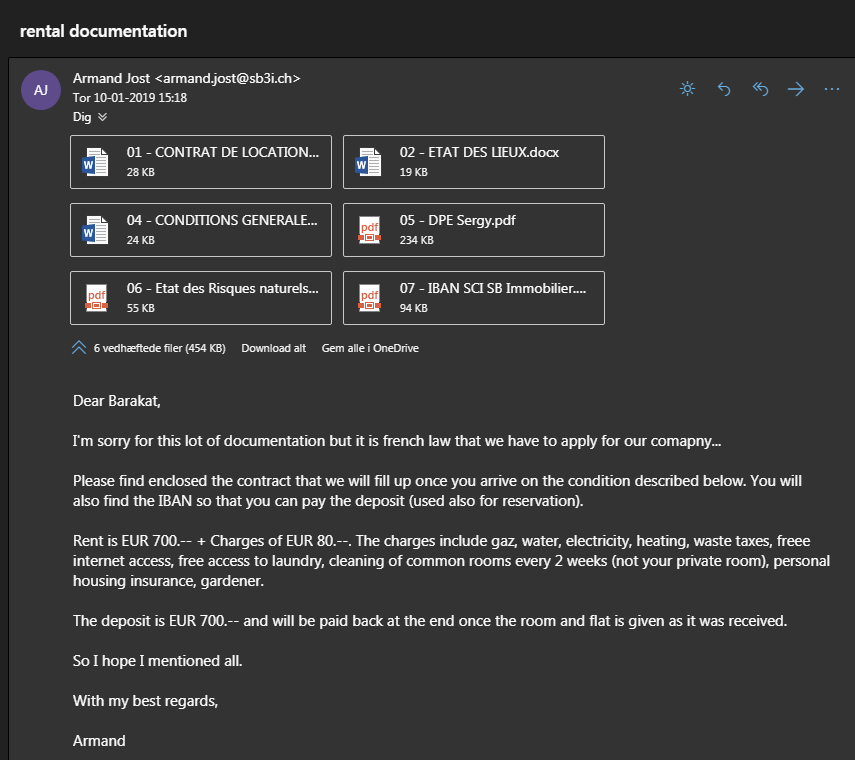
\includegraphics[width=1.0\textwidth]{Eksterne_filer/leje2.PNG}
\end{figure}
    \newpage
Herunder ses betalingen af huslejen for februar 2019 (inkl. 700 EUR depositum, derfor et samlet beløb på 1.480,00 EUR):
\begin{figure}[H]
	\centering
	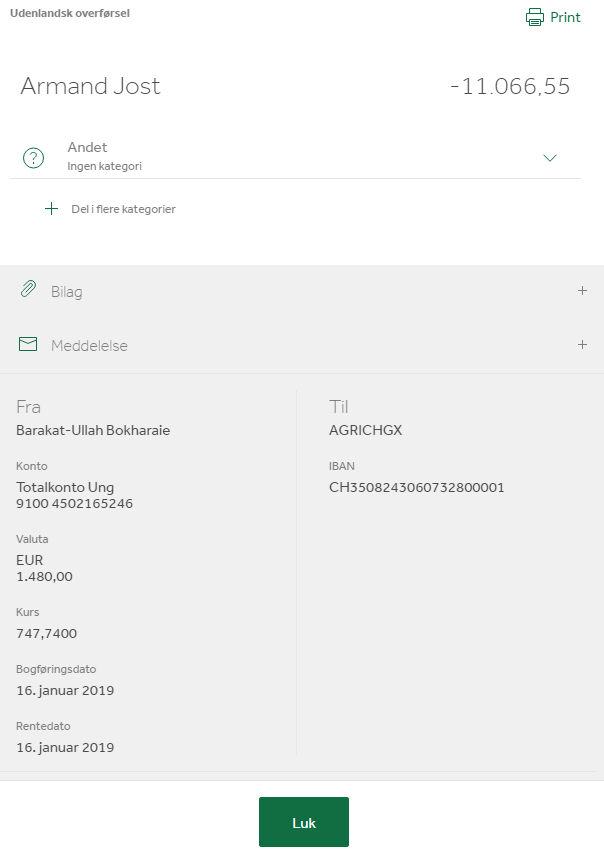
\includegraphics[width=0.8\textwidth]{Eksterne_filer/trans2.PNG}
\end{figure}
    \newpage

Herunder ses betalingen af den seneste husleje for marts 2019:
\begin{figure}[H]
	\centering
	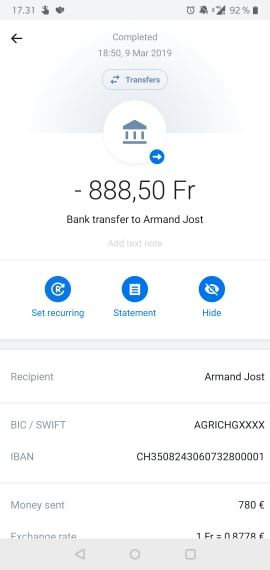
\includegraphics[width=0.5\textwidth]{Eksterne_filer/trans.jpg}
\end{figure}
\end{document}
